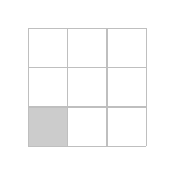
\begin{tikzpicture}[scale = 0.5]
    \def \Dx {12}
    \def \stp {1}
    \def \stpp {3}
  
    % style of grid
    \draw[fill=lightgray!80] (0,0) rectangle (\stp,\stp);
    \tikzset{gridstyle1/.style={color=lightgray,thin}}
    \draw[style=gridstyle1,step=\stp] (0,0) grid (\stpp,\stpp);
    \draw (\stp/2,\stp/2) node{$\volf$};
  
    % \draw plot coordinates{(\stp*2+\stp/2,\stp*2+\stp/2)} node[sloped] {$\Omega_{i}$};
    % \draw[line width=2pt,color=blue] (\Dx/2, 0) -- (0,0) -- (0,\Dx) -- (\Dx/2,\Dx);
    % \draw[line width=2pt,color=red] (\Dx/2, 0) -- (\Dx,0) -- (\Dx,\Dx) -- (\Dx/2,\Dx);
    % \draw[->, ultra thick] (-2,\Dx/2+1) node[sloped, left]{$\Gamma_{D}$} -- (0,\Dx/2);
    % \draw[->, ultra thick] (\Dx+2,\Dx/2+1) node[sloped, right]{$\Gamma_{N}$} -- (\Dx,\Dx/2);
    % \draw[fill=yellow!50] (0.5,0.5) circle (0.2);
    % \draw plot [mark=*, mark size=2] coordinates{(0.5,0.5)};
    % \draw[fill=yellow!50] (\Dx-0.5,\Dx-0.5) circle (0.2);
    % \draw plot [mark=*, mark size=2] coordinates{(\Dx-0.5,\Dx-0.5)};
    % \draw[->, ultra thick] (-1,1) node[sloped, left]{$\Gamma_{I}$} -- (0.5,0.5);
    % \draw[->, ultra thick] (\Dx+0.5,\Dx+0.5) node[sloped, right]{$\Gamma_{P}$} -- (\Dx-0.5,\Dx-0.5);
  
  \end{tikzpicture}
  